\chapter{5.Entrauschen: Filter und Co}
%This, again, is just a translation of my lecture note
%TODO move the tikz graphics into the dedicated directory
	\section{Noise}
		\mim{Noise} = Unwanted disturbances in an image. Mostly becaue of 
		\begin{enumerate}[-]
			\item point wise
			\item random
			\item independent
		\end{enumerate}
				We consider \emph{noise} to be an additive disturbances (for multiplicative noise use $log$).

		\emph{Notation:}
		\begin{center}
			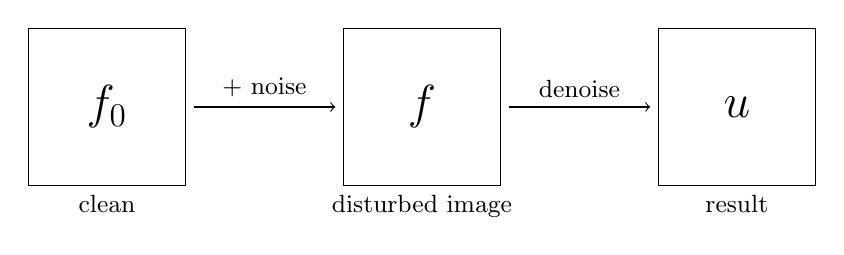
\begin{tikzpicture}
				\draw (0,0) rectangle (2,2);
				\draw (1,0) node[below] {\small clean};
				\draw (1,1) node[] {\LARGE $f_0$};
				\draw[->] (2.1,1) -- node[above] {\small $+$ noise} (3.9,1);
				\draw (4,0) rectangle (6,2);
				\draw (5,0) node[below] {\small disturbed image};
				\draw (5,1) node[] {\LARGE $f$};
				\draw[->] (6.1,1) -- node[above] {\small denoise} (7.9,1);
				\draw (8,0) rectangle (10,2);				
				\draw (9,0) node[below] {\small result};
				\draw (9,1) node[] {\LARGE $u$};
			\end{tikzpicture}
		\end{center}

		The quality of the denoised image $u$ compared to the original image $f_0$ is described by norms:
		\[
				\begin{aligned}
								\norm{f-f_0} & \dots \text{noise}\\
						\norm{u-f_0} & \dots \text{\mim{absolute error}}\\
						\frac{\norm{u-f_o}}{\norm{f-f_0}} & \dots \text{\mim{relative error} compared to the noise}\\
						\frac{\norm{u-f_o}}{\norm{f_0}} & \dots \text{relative error compared to the signal}
				\end{aligned}
				\]
		
		Typically the chosen norm is:
		\[\norm{f} = \norm{f}_2 = \sqrt{\int_{\Omega} \abs{f(x)}^2 dx}\]
		or in the discrete:
		\[\norm{f}_2=\sqrt{\sum_{x \in \Omega} \abs{f(x)}^2}\]

		Closely connected is the \mim{Signal to noise ratio} (SNR):
		\[log(\underbrace{\frac{\norm{f_0}_2}{\norm{u-f_0}_2}}_{\in \ [1,\infty)}) \in [0,+\infty), \text{ where $0$ is bad and $+\infty$ is good.}\]
	\section{smoothing filter}
		Idea: (to simplify in 1D)
		\begin{center}
			\begin{tikzpicture}
				\draw (0,0) node[left] {$f_0$:};
				\draw[thick] plot [smooth, tension = 0.7] coordinates {(0,0) (1.75,1.5) (3.5,0.5) (6,2) (9,0) (11,0.5)};
				\draw[->,thick] (-0.3,-0.5) -- node[left] {noise} (-0.3,-2);
				\draw (0,-2.5) node[left] {$f$:};				
				\draw[thick, name path = P2,shift = {(0,-2.5)}] plot [smooth, tension = 0.7] coordinates {(0,0) (1.75,1.5) (3.5,0.5) (6,2) (9,0) (11,0.5)};
				\draw[name path = P1, draw = none] (0,-1.1) -- (3,-1.1);
				\draw[name intersections={of = P1 and P2},red,thick]
				(intersection-1) edge[bend right] ++(0.3,0.5) ++(0.3,0.5) edge[bend right] (intersection-2);
				\draw[name path = P3,draw = none] (3,-2.3) -- (5,-1.2);
				\draw[name intersections={of = P3 and P2},red,thick]
				(intersection-1) edge[bend left] ++(0.3,-0.3) ++(0.3,-0.3) edge[bend left] (intersection-2);
				\draw[] (2,-0.9) -- ++(0.5,-0.1) node[right] {\small disturbances} (3.5,-2.1) -- ++(-0.5,0.9);
				\draw (0,-5) node[left] {$f$:};
				\draw[thick, name path = P4,shift = {(0,-5)}] plot [smooth, tension = 0.7] coordinates {(0,0) (1.75,1.5) (3.5,0.5) (6,2) (9,0) (11,0.5)};
				\draw[name path = P5, shift = {(0,-2.5)}, draw = none] (0,-1.1) -- (3,-1.1);
				\draw[name intersections={of = P4 and P5},red,thick]
				(intersection-1) edge[bend right] node[black,pos=0] {\small \textbullet} ++(0.3,0.5) ++(0.3,0.5) edge[bend right] node[black,pos=1] {\small \textbullet}  node[black,pos=0] {\small \textbullet} (intersection-2);
				\draw[name path = P6, shift = {(0,-2.5)}, draw = none] (3,-2.3) -- (5,-1.2);
				\draw[name intersections={of = P4 and P6},red,thick]
				(intersection-1) edge[bend left] node[black,pos=0] {\small \textbullet} ++(0.3,-0.3) ++(0.3,-0.3) edge[bend left] node[black,pos=1] {\small \textbullet}  node[black,pos=0] {\small \textbullet} (intersection-2);
				\draw[decorate,decoration={brace,amplitude=2pt,mirror}] (1.4,-3.7) -- (2.2,-3.7);
				\draw[thick] (1.8,-3.8) -- (1.8,-4.3) node[below] {\small \framebox{average}};
				\draw[->,thick,double] (1.6,-5) -- (0.4,-5);
				\draw[->,thick,double] (2,-5) -- (3.2,-5);
				\draw[->,thick] (1.8,-5.1) -- (1.8,-5.7);
				\draw (0,-7.5) node[left] {$u$:};
				\draw[->,thick] (-0.3,-5.5) -- node[left] {denoising} (-0.3,-7);
				\draw[thick, name path = P7,shift = {(0,-7.5)}] plot [smooth, tension = 0.7] coordinates {(0,0) (1.75,1.5) (3.5,0.5) (6,2) (9,0) (11,0.5)};
				\draw[name path = P8, shift = {(0,-5)}, draw = none] (0,-1.2) -- (3,-1.2);
				\draw[name intersections={of = P7 and P8},red,thick]
				plot [smooth,tension=0.7] coordinates {(intersection-1) ($(intersection-1) + (0.5,0.35)$) (intersection-2)};
				\draw[name path = P9, shift = {(0,-5)}, draw = none] (3,-2.25) -- (5,-1.15);
				\draw[name intersections={of = P7 and P9},red,thick]
				plot [smooth,tension=0.7] coordinates {(intersection-1) ($(intersection-1) + (0.45,0.05)$) (intersection-2)};
			\end{tikzpicture}
		\end{center}

		\begin{equation} \label{eq:5.1}
			u(k):=\alpha \cdot f(k-1) + \beta \cdot f(k) + \gamma \cdot f(k+1)
		\end{equation}
		where:
		\begin{equation} \label{eq:5.2}
			\alpha + \beta + \gamma = 1
		\end{equation}

		More precisely \eqref{eq:5.1} means:
		
		\begin{center}
			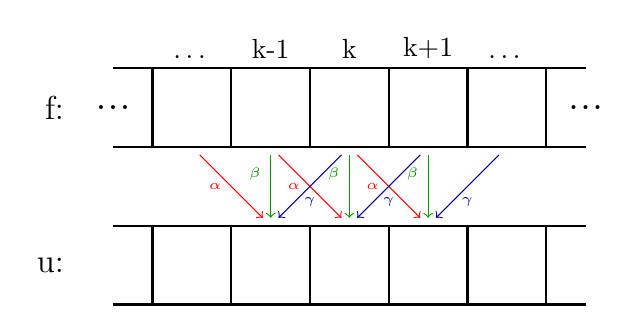
\begin{tikzpicture}
				\draw (0,-0.5) node[left] {\large f:};
				\draw[thick] (0.5,0) grid (6.5,-1);
				\draw (0.5,-0.5) node {\LARGE ...};
				\draw (6.5,-0.5) node {\LARGE ...};
				\draw (1.5,0) node[above] {\dots};
				\draw (2.5,0) node[above] {k-1};
				\draw (3.5,0) node[above] {k};
				\draw (4.5,0) node[above] {k+1};
				\draw (5.5,0) node[above] {\dots};

				\draw[->,red] (1.6,-1.1) -- node[left] {\tiny $\alpha$} (2.4,-1.9);
				\draw[->,red] (2.6,-1.1) -- node[left] {\tiny $\alpha$} (3.4,-1.9);
				\draw[->,red] (3.6,-1.1) -- node[left] {\tiny $\alpha$} (4.4,-1.9);
				\draw[->,black!40!green] (2.5,-1.1) -- node[left, pos = 0.3] {\tiny $\beta$} (2.5,-1.9);
				\draw[->,black!40!green] (3.5,-1.1) -- node[left, pos = 0.3] {\tiny $\beta$} (3.5,-1.9);
				\draw[->,black!40!green] (4.5,-1.1) -- node[left, pos = 0.3] {\tiny $\beta$} (4.5,-1.9);
				\draw[->,black!40!blue] (3.4,-1.1) -- node[right, pos = 0.75] {\tiny $\gamma$} (2.6,-1.9);
				\draw[->,black!40!blue] (4.4,-1.1) -- node[right, pos = 0.75] {\tiny $\gamma$} (3.6,-1.9);
				\draw[->,black!40!blue] (5.4,-1.1) -- node[right, pos = 0.75] {\tiny $\gamma$} (4.6,-1.9);

				\draw (0,-2.5) node[left] {\large u:};
				\draw[thick] (0.5,-2) grid (6.5,-3);
			\end{tikzpicture}
		\end{center}

		\begin{center}
			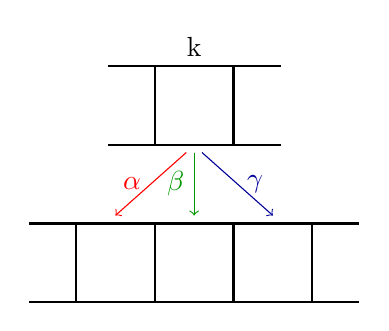
\begin{tikzpicture}
				\draw (0.5,0) node[above] {k};
				\draw[thick] (-0.6,0) grid (1.6,-1);
				\draw[->,red] (0.4,-1.1) -- node[left] {$\alpha$} (-0.5,-1.9);
				\draw[->,black!40!green] (0.5,-1.1) -- node[left] {$\beta$} (0.5,-1.9); 
				\draw[->,black!40!blue] (0.6,-1.1) -- node[right] {$\gamma$} (1.5,-1.9); 
				\draw[thick] (-1.6,-2) grid (2.6,-3);
			\end{tikzpicture}
		\end{center}

		With \eqref{eq:5.1} there is a mapping $f \mapsto u$, we write
		\[u = m \boxast f, \ \text{this is called \mim{Correlation}.}\]%TODO is it really correlation?
		where:
		\begin{equation}\label{eq:5.3}
			\framebox{$\displaystyle (m \boxast f)(k) = \sum_{i \in supp(m)} m(i) f(k+i)$}
		\end{equation}
		and:
		\begin{center}
			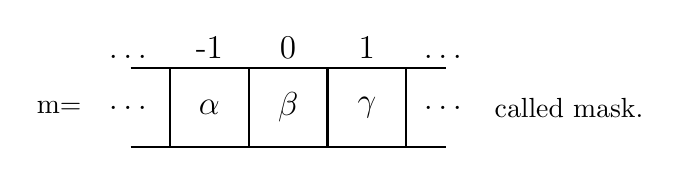
\begin{tikzpicture}
				\draw (0,0.5) node[left] {m=};
				\draw[thick] (0.5,0) grid (4.5,1);
				\draw (0.5,0.5) node {\large \dots};
				\draw (1.5,0.5) node {\large $\alpha$};
				\draw (2.5,0.5) node {\large $\beta$};
				\draw (3.5,0.5) node {\large $\gamma$};				
				\draw (4.5,0.5) node {\large \dots};
				\draw (0.5,1) node[above] {\large \dots};
				\draw (1.5,1) node[above] {\large -1};
				\draw (2.5,1) node[above] {\large 0};
				\draw (3.5,1) node[above] {\large 1};				
				\draw (4.5,1) node[above] {\large \dots};
				\draw (5,0.5) node[right] {called \mim{mask}.};
			\end{tikzpicture}
		\end{center}

		If you set $j:= k + i$ in \eqref{eq:5.1}, then $i=j-k$, which means:
		\begin{equation}\label{eq:5.4}
			\framebox{$\displaystyle (m \boxast f)(k) = \sum_{i \in supp(m)} m(j-k) f(j)$}
		\end{equation}

		To apply the mapping onto the boundary the image is reflected, in 1D:
		\begin{center}
			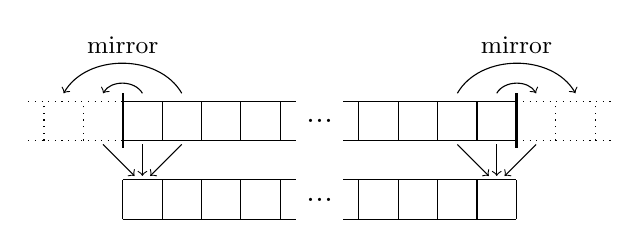
\begin{tikzpicture}
				\draw[step = 0.5] (0,0) grid (2.2,-0.5);
				\draw (2.5,-0.25) node {\large ...};
				\draw[step = 0.5] (2.8,0) grid (5,-0.5);
				\draw[thick] (0,0.1) -- (0,-0.6);
				\draw[thick] (5,0.1) -- (5,-0.6);
				\draw[step = 0.5, dotted] (0,0) grid (-1.2,-0.5);
				\draw[step = 0.5, dotted] (5,0) grid (6.2,-0.5);
				\draw[] (0.25,0.1) edge[bend right = 60, ->] (-0.25,0.1);
				\draw[] (0.75,0.1) edge[bend right = 60, ->] node[above] {\small mirror} (-0.75,0.1);
				\draw[] (4.75,0.1) edge[bend left = 60, ->] (5.25,0.1);
				\draw[] (4.25,0.1) edge[bend left = 60, ->] node[above] {\small mirror} (5.75,0.1);
				\draw[step = 0.5] (0,-1) grid (2.2,-1.5);
				\draw (2.5,-1.25) node {\large ...};
				\draw[step = 0.5] (2.8,-1) grid (5,-1.5);
				\draw[->] (0.25,-0.55) -- (0.25,-0.95);
				\draw[->] (-0.25,-0.55) -- (0.15,-0.95);
				\draw[->] (0.75,-0.55) -- (0.35,-0.95);
				\draw[->] (4.75,-0.55) -- (4.75,-0.95);
				\draw[->] (4.25,-0.55) -- (4.65,-0.95);
				\draw[->] (5.25,-0.55) -- (4.85,-0.95);
			\end{tikzpicture}
		\end{center}

		in 2D:

		\begin{center}
			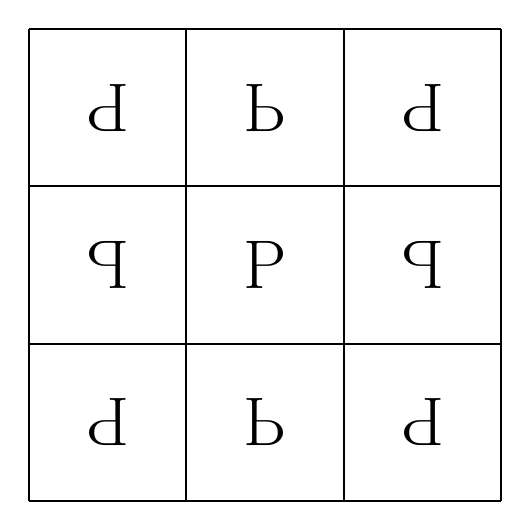
\begin{tikzpicture}
				\draw[step =2, thick] (0,0) grid (6,6);
				\draw (3,3) node {\Huge P};
				\draw (1,1) node[rotate = 180] {\Huge P};
				\draw (5,1) node[rotate = 180] {\Huge P};
				\draw (1,5) node[rotate = 180] {\Huge P};
				\draw (5,5) node[rotate = 180] {\Huge P};
				\draw (3,5) node[yscale=-1,xscale=1] {\Huge P};
				\draw (5,3) node[rotate = 180,yscale=-1,xscale=1] {\Huge P};
				\draw (1,3) node[rotate = 180,yscale=-1,xscale=1] {\Huge P};
				\draw (3,1) node[yscale=-1,xscale=1] {\Huge P};
			\end{tikzpicture}
		\end{center}

		Formula \eqref{eq:5.4} might remind one of the \mim{convolution}:
		\todoLayout
		\begin{equation}\label{eq:5.5}
			\framebox{$\displaystyle (g * f)(k) = \sum_{j \in \Z} g(\underbrace{k-j}_{\text{Difference to \eqref{eq:5.4}}}) \cdot f(j)$}
		\end{equation}

		If you set $g(i) := m(-i) =: \tilde m(i)$, which corresponds to 
		a reflection of the Mask, then
		\[m \boxast f = g * f = \tilde m * f\]
		\todoKom{Im Skript hier noch Beispiele und soetwas p. 32f}
		Properties of the convolution:
		\begin{enumerate}
			\item $(f * g) * h = f * (g* h)$, Associativity
			\item $f*g=g*f$, Commutativity
			\item $\tilde f * \tilde g = \widetilde{f * g}$, 
				Compatibility with reflection
		\end{enumerate}
		
		Properties of the correlation:
		\begin{enumerate}
			\item $f \boxast (g \boxast h) = \tilde f * ( \tilde g* h) 
				\overset{\framebox{\small 1}}{=} ( \tilde f * \tilde g) * h
				\overset{\framebox{\small 3}}{=} (\widetilde{f * g}) * h = 
				(f * g) \boxast h \neq (f \boxast g) \boxast h$, not associative!
			\item $f \boxast g = \tilde f * g \overset{
				\framebox{\small 2}}{=} g * \tilde f = 
					\tilde{\tilde g} * \tilde f \overset{\framebox{\small 3}}{=}
					\widetilde{(\tilde g * f)} = 
					\widetilde{g \boxast f} \neq g \boxast f$, not commutative!
			\item $\tilde f \boxast \tilde g = 
				\tilde{\tilde f} * \tilde g \overset{\framebox{\small 3}}{=}
				\widetilde{(\tilde f * g)} = \widetilde{f \boxast g}$, 
				Compatibility with reflection
		\end{enumerate}

		$\boxast$ und $*$ definiert man auf: 
			$\ell^1(\Z^d):=\set{f=(f_i)_{i \in \Z^d} : \underbrace{\sum_{
				i \in \Z^d}\abs{f_i}}_{:=\norm{f}_1} < \infty}$
		
			Man kann zeigen (Übung): $f,g \in \ell^1 \Rightarrow f * g \in \ell^1$ 
			und $\norm{f * g}_1 \leq \norm{f}_1 \cdot \norm{g}_1$.
			Wobei oft die Gleichheit gilt.
			
			Alles gilt auch in der Kontinuierlichen Version:
			\[L^1(\R^d) := \set{f:\R^d \to \R : 
				\underbrace{\int_{\R^d}\abs{f} dx}_{:=\norm{f}_1} < \infty} \]
			\[f,g \in L^1(\R^d): (g*f)(x)=\int_{\R^d}g(x-y)f(y) dy, \ y,x \in \R^d\]
		
			Beispiel für den kontinueirlichen Fall:
			\begin{center}
				\begin{tikzpicture}
					\draw[dotted] (0,1) node[left] {$\frac{1}{2a}$} -- (8,1);
					\draw (0,0) node[left] {$g:$} -- (2.5,0) -- (2.5,1) -- (5.5,1) -- (5.5,0) -- (8,0);
					\draw (2.5,0) node[below] {\small $-a$};
					\draw[dotted] (4,0) node[below] {\small $0$} -- (4,1.5);
					\draw (5.5,0) node[below] {\small $-a$};
				\end{tikzpicture}
			\end{center}
			Hierbei gilt $\displaystyle \int_{\R} g(x) dx = 1$
		
			\begin{center}
				\begin{tikzpicture}
					\draw[thick, name path = P2,shift = {(0,-2.5)}] node [left] {$f:$}plot [smooth, tension = 0.45] coordinates {(0,0) (1.2,1.5) (2.1,0.3) (3,2) (4.3,1) (5.3,1.6) (6.6,0.5) (7.5,1) (8,0)};
				\end{tikzpicture}
			\end{center}
		
			$g \boxast f = $ \mim{gleitendes Mittel}.\\
		
				\begin{tikzpicture}
					\draw[dotted] (0,1) node[left] {$\frac{1}{2a}$} -- (8,1);
					\draw (0,0) node[left] {$g \boxast g = \tilde g * g = g * g=$} -- (1,0) -- (4,1) -- (7,0) -- (8,0);
					\draw (1,0) node[below] {\small $-2a$};
					\draw[dotted] (4,0) node[below] {\small $0$} -- (4,1.5);
					\draw (7,0) node[below] {\small $-2a$};
				\end{tikzpicture}
		
			\todoLayout
			Weitere Eigenschaften der Faltung:\\
			Für alle $f,g \in L^1$ or $\ell ^1$
			\begin{equation*}
				\left.\begin{aligned}
					(g_1 + g_2) * f = (g_1 * f) + (g_2 * g)\\
					(\alpha g) * f = \alpha (g * f)
				\end{aligned}\right\}=\text{Linearität}
			\end{equation*}
			Somit ist:
			\[g \mapsto f * g\]
			ein linearer Operator.
		
			Formt $\ell^1$ bzw. $L^1$ eine Algebra mit neutralem Element $\delta$?
		
			$\ell^1$?:
			\begin{center}
				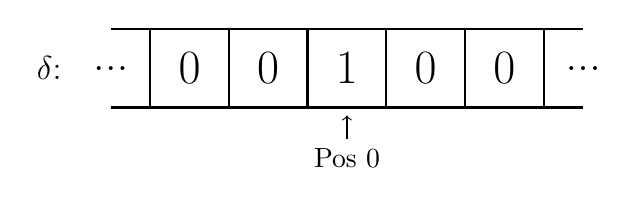
\begin{tikzpicture}
					\draw (0,-0.5) node[left] {\large $\delta$:};
					\draw[thick] (0.5,0) grid (6.5,-1);
					\draw (0.5,-0.5) node {\LARGE ...};
					\draw (6.5,-0.5) node {\LARGE ...};
					\draw (1.5,-0.5) node {\LARGE 0};
					\draw (2.5,-0.5) node {\LARGE 0};
					\draw (3.5,-0.5) node {\LARGE 1};
					\draw (4.5,-0.5) node {\LARGE 0};
					\draw (5.5,-0.5) node {\LARGE 0};
					\draw[->] (3.5,-1.4) node[below] {Pos $0$} -- (3.5,-1.1);
				\end{tikzpicture}
			\end{center}
			Ja!
		
			$L^1$?:
			Für ein solches Element muss gelten:\\
			$\forall f \in L^1 : d * f = f$\\
			$\forall x \in \R :\displaystyle \int_{\R^d} \underbrace{\delta(x-y)}_{=0 \forall x \neq y} f(y) dy = f(x)$
		
			Diese Funktion wird \mim{Dirac-Impuls} gennant ist aber kein Element von $L^1$.
		
			\underline{Nun zu Masken in 2D:}
		
			\begin{equation*}
				u = m \boxast f \text{ mit } m= \raisebox{-0.665cm}{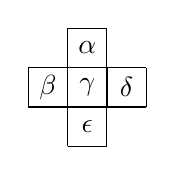
\begin{tikzpicture}
					\draw[step = 0.5] (0,0) grid (0.5,1.5);
					\draw[step = 0.5] (-0.5,1) grid (1,0.5);
					\draw (0.25,1.25) node {$\alpha$};
					\draw (0.25,0.75) node {$\gamma$};
					\draw (0.25,0.25) node {$\epsilon$};
					\draw (-0.25,0.75) node {$\beta$};
					\draw (0.75,0.75) node {$\delta$};
				\end{tikzpicture}}
			\end{equation*}
			wobei $\alpha + \beta +\gamma +\delta + \epsilon = 1$\\
			Kurzschreibweise: $u_{ij}:=u(x)$ wobei $x = \begin{pmatrix}i\\j\end{pmatrix} \in \Z^2$, analog für $f_{ij}$.
		
			\[\Rightarrow u_{ij} = \alpha f_{i-1,j} + \beta f_{i,j-i} + \gamma f_{ij} + \delta f_{i,j+1} + \epsilon f_{i+1,j}\]
		
			\begin{equation*}
				u = m \boxast f = \tilde m * f \text{ mit } \tilde m = \raisebox{-0.665cm}{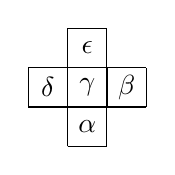
\begin{tikzpicture}
					\draw[step = 0.5] (0,0) grid (0.5,1.5);
					\draw[step = 0.5] (-0.5,1) grid (1,0.5);
					\draw (0.25,1.25) node {$\epsilon$};
					\draw (0.25,0.75) node {$\gamma$};
					\draw (0.25,0.25) node {$\alpha$};
					\draw (-0.25,0.75) node {$\delta$};
					\draw (0.75,0.75) node {$\beta$};
				\end{tikzpicture}}
			\end{equation*}
		
			\underline{Symmetrischer Fall:}
		
			\begin{equation*}
			\tilde m = \raisebox{-0.665cm}{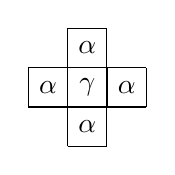
\begin{tikzpicture}
					\draw[step = 0.5] (0,0) grid (0.5,1.5);
					\draw[step = 0.5] (-0.5,1) grid (1,0.5);
					\draw (0.25,1.25) node {$\alpha$};
					\draw (0.25,0.75) node {$\gamma$};
					\draw (0.25,0.25) node {$\alpha$};
					\draw (-0.25,0.75) node {$\alpha$};
					\draw (0.75,0.75) node {$\alpha$};
				\end{tikzpicture}} \text{ mit } \gamma = 1 - 4 \alpha
			\end{equation*}
		
			\begin{equation}
				u_{ij} = (1 - 4 \alpha)f_{ij} + \alpha(f_{i-1,j} + f_{i,j-1} + f_{i,j+1} + f_{i+1,j})
			\end{equation}
		
			\begin{equation*}
					\text{Erinnerung: } \raisebox{-1.2cm}{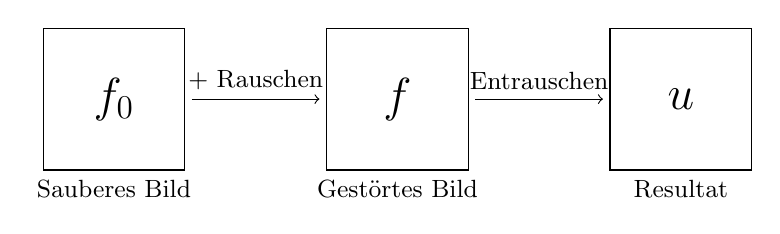
\begin{tikzpicture}[scale=0.9]
						\draw (0,0) rectangle (2,2);
						\draw (1,0) node[below] {\small Sauberes Bild};
						\draw (1,1) node[] {\LARGE $f_0$};
						\draw[->] (2.1,1) -- node[above] {\small $+$ Rauschen} (3.9,1);
						\draw (4,0) rectangle (6,2);
						\draw (5,0) node[below] {\small Gestörtes Bild};
						\draw (5,1) node[] {\LARGE $f$};
						\draw[->] (6.1,1) -- node[above] {\small Entrauschen} (7.9,1);
						\draw (8,0) rectangle (10,2);				
						\draw (9,0) node[below] {\small Resultat};
						\draw (9,1) node[] {\LARGE $u$};
					\end{tikzpicture}}
			\end{equation*}
		
			Annahme: $f_{ij} = f_{ij} +r_{ij}$ mit $r_{ij} \sim N(0,\sigma^2)$ iid.
		
			z.z.: $Var(u_{ij}) \leq Var(f_{ij})$\\
			
			\begin{equation*}
				Var(f_{ij}) = E(\underbrace{f_{ij} - \overbrace{E f_{ij}}^{f^0_{ij}}}%
					_{r_{ij}})^2 = \sigma^2
			\end{equation*}
		
			\todoLayout
			\begin{align*}
				Var(u_{ij}) &= E(u_{ij} - E u_{ij})^2 = E((1 - 4 \alpha) (\underbrace{f_{ij} - f^0_{ij}}_{r_{ij}}) + \alpha(\underbrace{(f_{i-1,j} - f^0_{i-1,j})}_{r_{i-1,j}} + ... + \underbrace{(f_{i+1,j} - f^0_{i+1,j})}_{r_{i+1,j}}))^2\\
				&= E((1 - 4 \alpha)^2 r_{ij}^2 + \alpha^2(r_{i-1,j}^2 + r_{i,j-1}^2 +r_{i,j+1}^2 + r_{i+1,j}^2) + 2 (1 - 4 \alpha) \alpha r_{ij} r_{i-1,j}...)\\
				&= (1 - 4 \alpha)^2 \underbrace{E r_{i,j}^2}_{\sigma^2} + \alpha^2(E r_{i-1,j}^2 + ... + E r_{i+1,j}^2) + 2 (1 - 4 \alpha) \alpha \underbrace{E(r_{ij}r_{i-1,j})}_{\underbrace{E r_{ij} E r_{i-1,j}}_{0}} + \underbrace{...}_{0})\\
				&=(1 - 4 \alpha)^2 \sigma^2 + \alpha^2 4 \sigma^2 = (1 - 8 \alpha + 16 \alpha ^2 + 4 \alpha^2) \sigma^2
			\end{align*}
		
			Da $0 \leq \alpha$ und $ 0 \leq 1 - 4 \alpha \Rightarrow 0 \leq \alpha \leq \frac{1}{4}$:
		
			\begin{equation*}
				(1 - 8 \alpha + 16 \alpha ^2 + 4 \alpha^2) \sigma^2 = \underbrace{1 + \underbrace{20 \alpha}_{\geq 0} (\underbrace{\alpha - \frac{2}{5}}_{< 0})}_{\leq 1}
			\end{equation*}
		
			$\Rightarrow Var(u_{ij}) \leq Var(f_{ij})$ für $\alpha \in [0,\frac{1}{4}]$\\
			
			Dabei gilt: $Var(u_{ij}) \overset{\alpha}{\to} d \text{min} \iff 1 - 8 \alpha + 20 \alpha^2 \overset{\alpha}{\to} \text{min} \iff -8 + 40 \alpha = 0 \iff \alpha = \frac{1}{5}$
		
			\begin{equation*}
				\Rightarrow \text{bester Filter} : \ \raisebox{-0.9cm}{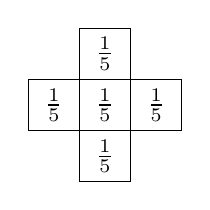
\begin{tikzpicture}[scale = 1.3]
						\draw[step = 0.5] (0,0) grid (0.5,1.5);
						\draw[step = 0.5] (-0.5,1) grid (1,0.5);
						\draw (0.25,1.25) node {$\frac{1}{5}$};
						\draw (0.25,0.75) node {$\frac{1}{5}$};
						\draw (0.25,0.25) node {$\frac{1}{5}$};
						\draw (-0.25,0.75) node {$\frac{1}{5}$};
						\draw (0.75,0.75) node {$\frac{1}{5}$};
					\end{tikzpicture}}
				\end{equation*}

\todoKom{Kapitel sollte noch fehlergelesen werden. 
	Es könnte noch einiges aus dem Skript übernommen werden. 
	Es braucht etwas Layout }

\section{Frequenzfilter}
	\emph{Ansatz}: Rauschen $\approx$ hochfrequente Anteile des Bildes/Signals\\
	\hspace{0.5\linewidth} $\df$ gezieltes entfernen

	\newcommand{\skprod}[2]{
		\left \langle #1,#2 \right \rangle
	}
	\newcommand{\srmatrix}[1] {
	\left( \begin{smallmatrix} #1 \end{smallmatrix} \right)
	}

Wichtiges Instrument: Fouriertransformation (FT)

$$ \mathcal{F} : f \mapsto \hat{f} \text{ mit } \hat{f} (z) = 
	\frac{1}{(2\pi^{\frac{d}{2}}}  \int_{\R^d}dx$$

\todoKom{hier fehlt der rest aus einer Vorlesung}

\todoKom{siehe auch p. 41}

\begin{equation*}
	\begin{tikzpicture}[scale = 0.9]
		\draw (0,0) rectangle (2,2);
		\draw (1,0) node[below] {\small Sauberes Bild};
		\draw (1,1) node[] {\LARGE $f_0$};
		\draw[->] (2.1,1) -- node[above] {$+r$} (2.9,1);
		\draw (3,0) rectangle (5,2);
		\draw (4,0) node[below] {\small Gestörtes Bild};
		\draw (4,1) node[] {\LARGE $f$};
		\draw[->] (5.1,1) -- node[above] {$\mathcal F$} (5.9,1);
		\draw (6,-0.5) rectangle (9,2.5);
		\draw (6,1) -- (9,1);
		\draw[thick, name path = P2]plot [smooth, tension = 0.8] coordinates {(6,1) (6.1,1.3) (6.4,1.1) (6.6,1.6) (7,1.1) (7.3,2.0) (7.5,1.1) (7.7,1.2) (7.8,1.9) (8.1,1.5) (8.5,1.9) (9,1)};
		\draw[->] (9.1,1) -- node[above] {\small Abschneiden} (10.9,1);
		\draw[->] (14.1,1) -- node[above] {$\mathcal F^{-1}$} (14.9,1);
		\draw[decorate,decoration={brace,amplitude=2pt,mirror}] (6,0.6) -- node[below] {\scriptsize \begin{tabular}{c} niedrige \\ Frequenzen \end{tabular}} (7.5,0.6);
		\draw[decorate,decoration={brace,amplitude=2pt,mirror}] (7.5,0.6) -- node[below] {\scriptsize \begin{tabular}{c} hohe \\ Frequenzen \end{tabular}} (9,0.6);
		\draw[thick, name path = P2,shift = {(5,0)}]plot [smooth, tension = 0.8] coordinates {(6,1) (6.1,1.3) (6.4,1.1) (6.6,1.6) (7,1.1) (7.3,2.0) (7.5,1.1) (7.7,1.2) (7.8,1.9) (8.1,1.5) (8.5,1.9) (9,1)};
		\draw[color = white,fill] (12.7,1) rectangle (14,2.5);
		\draw (11,1) -- (14,1);                
		\draw (11,-0.5) rectangle (14,2.5);
		\draw (15,0) rectangle (17,2);
		\draw[thick] (7.7,0.8) -- (7.7,2.3);
		\draw[thick] (12.7,0.8) -- (12.7,2.3);                
		\draw (16,1) node[] {\LARGE $u$};
		\draw[decorate,decoration={brace,amplitude=2pt,mirror}] (5.5,-1) -- node[below] {im Frequenzbereich} (14.5,-1);
		\draw[decorate,decoration={brace,amplitude=2pt,mirror}] (3,-1.5) -- node[below] {\mim{Frequenzraumfilter} (Tiefpass)} (17,-1.5);
	\end{tikzpicture}
\end{equation*}

Wobei  $z \in \R^d, f \in L^1(\R^d)$.

    Falls auch $\hat f \in L^1(\R^d)$ ist ,dann lässt sich $f$ wie folgt mittels der inversen Fouriertransformation aus $\hat f$ rekonstruieren:

    \[\mathcal F^{-1} : \hat f \mapsto f\]
    \begin{equation}
        \boxed{\hat f(z) = \frac{1}{(2 \pi)^\frac{d}{2}} \int_{\R^d} f(x) e^{i \skprod{z}{x}} dx}
    \end{equation}
    Wobei $x \in \R^d$.\\

    Man hat also $\mathcal F^{-1} \mathcal F f$, d.h.

    \[f(x) = \frac{1}{(2 \pi)^\frac{d}{2}} \int_{\R^d} \left(\frac{1}{(2 \pi)^\frac{d}{2}} \int_{\R^d} f(y) e^{-i \skprod{z}{y}} dy\right) e^{i \skprod{z}{x}} dz\]

    Sei nun $e_z(x) := e^{i \skprod{z}{x}}, \ x \in \R^d$ mit Parameter
$z = \srmatrix{z_1 \\ \vdots \\ z_d}$.\\
    Also $e_z(x) = e^{i\skprod{\srmatrix{z_1\\z_2}}{\srmatrix{x_1\\x_2}}} = e^{i (z_1 x_1 +z_2 x_2)}$\\
    Beispiele in $2D$:\\
    (Hier stellen die Linien, Punkte mit konstantem wert dar)

    \begin{minipage}[t]{0.49\linewidth}
        \begin{center}
            $z = \srmatrix{1 \\ 0}, \  e_z(x)=e^{ix_1}$:\\
            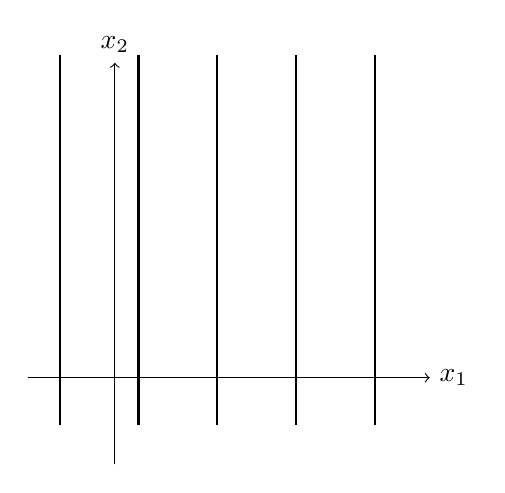
\begin{tikzpicture}
                \draw[->] (-1.1,0) -- (4,0) node[right] {$x_1$};
                \draw[->] (0,-1.1) -- (0,4) node[above] {$x_2$};
                \foreach \i in {-0.7, 0.3, 1.3, 2.3, 3.3}{
                    \draw[thick] (\i,-0.6) -- (\i,4.1);
                }
            \end{tikzpicture}

            $z = \srmatrix{0 \\ 1}, \  e_z(x)=e^{ix_2}$:\\
            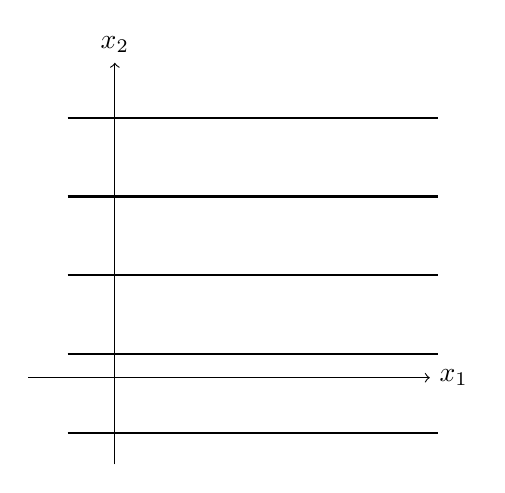
\begin{tikzpicture}
                \draw[->] (-1.1,0) -- (4,0) node[right] {$x_1$};
                \draw[->] (0,-1.1) -- (0,4) node[above] {$x_2$};
                \foreach \i in {-0.7, 0.3, 1.3, 2.3, 3.3}{
                    \draw[thick] (-0.6,\i) -- (4.1,\i);
                }
            \end{tikzpicture}

            $z = \srmatrix{1 \\ 1}, \  e_z(x)=e^{i(x_1 + x_2}$:\\
            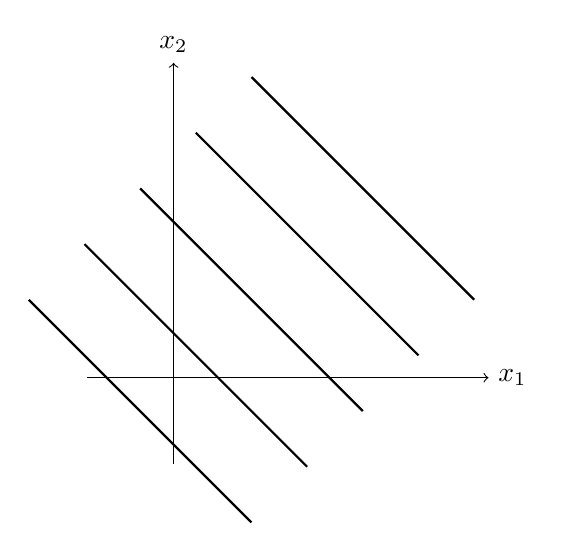
\begin{tikzpicture}
                \draw[->] (-1.1,0) -- (4,0) node[right] {$x_1$};
                \draw[->] (0,-1.1) -- (0,4) node[above] {$x_2$};
                \foreach \i in {-2.6, -1.6, -0.6, 0.4, 1.4}{
                    \draw[thick, rotate = -45,shift={(0,\i)}] (-2,2) -- (2,2);
                }
            \end{tikzpicture}
        \end{center}
    \end{minipage}
    \hfill
    \begin{minipage}[t]{0.49\linewidth}
        $z = \srmatrix{2 \\ 0}, \ e_z(x)=e^{i2x_1}$:\\
        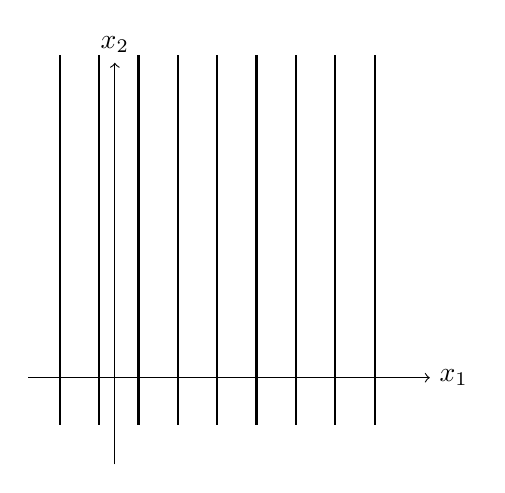
\begin{tikzpicture}
            \draw[->] (-1.1,0) -- (4,0) node[right] {$x_1$};
            \draw[->] (0,-1.1) -- (0,4) node[above] {$x_2$};
            \foreach \i in {-0.7, -0.2, 0.3, 0.8, 1.3, 1.8, 2.3, 2.8, 3.3}{
                \draw[thick] (\i,-0.6) -- (\i,4.1);
            }
        \end{tikzpicture}

        $z = \srmatrix{0 \\ 2}, \  e_z(x)=e^{i2x_2}$:\\
        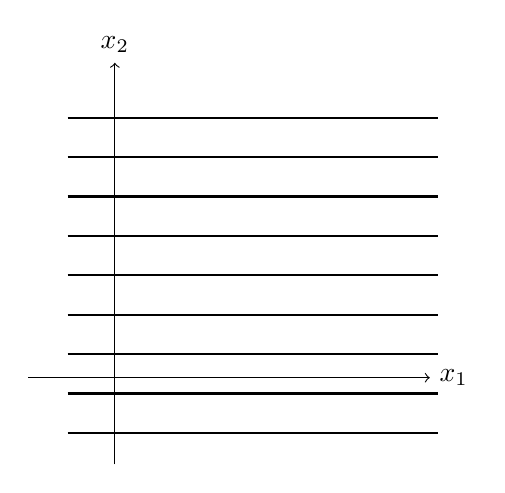
\begin{tikzpicture}
            \draw[->] (-1.1,0) -- (4,0) node[right] {$x_1$};
            \draw[->] (0,-1.1) -- (0,4) node[above] {$x_2$};
            \foreach \i in {-0.7, -0.2, 0.3, 0.8, 1.3, 1.8, 2.3, 2.8, 3.3}{
                \draw[thick] (-0.6,\i) -- (4.1,\i);
            }
        \end{tikzpicture}

        $z = \srmatrix{-2 \\ 1}, \  e_z(x)=e^{i(-2x_1 + x_2)}$:\\
        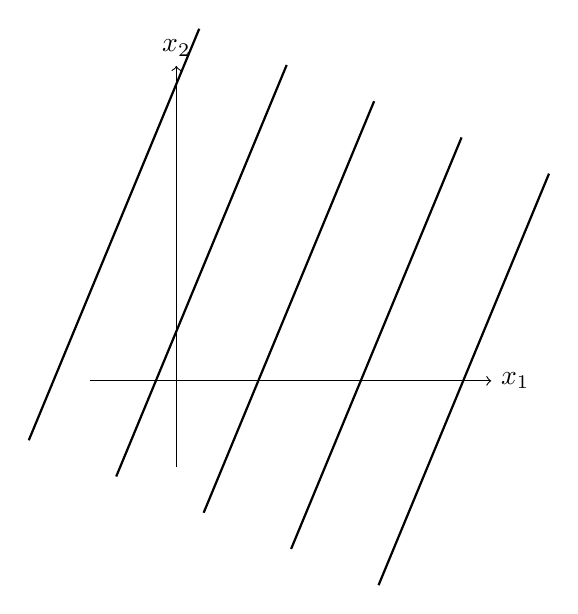
\begin{tikzpicture}
            \draw[->] (-1.1,0) -- (4,0) node[right] {$x_1$};
            \draw[->] (0,-1.1) -- (0,4) node[above] {$x_2$};
            \foreach \i in {-2.8, -1.8, -0.8, 0.2, 1.2}{
                \draw[thick, rotate = 112.5,shift={(0.85*\i,0.85*\i)}] (-1,1) -- (3,-3);
            }
        \end{tikzpicture}
    \end{minipage}
    
    $\displaystyle f \in L^2(\R^d) = \{f:\R^d \to \R | \int_{\R^d} \abs{f}^2 dx < \infty\}$ ist
    \begin{enumerate}[-]
        \item ein normierter Raum mit $+$, $\alpha \cdot$ und $\displaystyle \norm{\cdot}_2 := \sqrt{\int_{\R^d} \abs{f(x)}^2 dx}$
        \item ein Skalarproduktraum mit $\displaystyle \skprod{f}{g} := \int_{\R^d} f \bar g dx$, wobei $\norm{f}_2^2=\skprod{f}{f}$
        \item ein vollständiger Raum, also \mim{Banachraum}
    \end{enumerate}
    Ein vollständiger normierter Banachraum mit Skalarproduk heißt \mim{Hilbertraum}.

    $\mathcal F$ kann auch als Abbildung auf $L^2(\R^d)$ betrachtet werden. Dann gilt:\\
    \[\hat f = \mathcal F f \in L^2(\R^d)\]
    und
    \begin{equation}
        \norm{\hat f}_2 = \norm{f}_2
    \end{equation}
    und sogar
    \begin{equation}
        \skprod{\hat f}{\hat g}_2 = \skprod{f}{g}_2
    \end{equation}
    für alle $f,g \in L^2(\R^d)$.

    Weitere Eigenschaften der Fouriertransformation:

    \begin{enumerate}[-]
        \item $f \in L^1(\R^d) \Rightarrow \hat f$ stetig und $\underset{\abs{z} \to \infty}{lim} \hat f(z) = 0$
        \item $\mathcal F: L^1(\R^d) \to C(\R^d)$ ist eine lineare Abbildung
        \item $\mathcal F: L^1(\R^d) \to C(\R^d)$ ist eine beschränkte/stetige Abbildung
        \item Verschiebung $\overset{\mathcal F}{\to}$ Modulation, d.h.
        \begin{equation*}
            g(x) = f(x+a) \Rightarrow \hat g(z) = e^{i \skprod{a}{z}} \hat f(z)
        \end{equation*}
        \item Modulation $\overset{\mathcal F}{\to}$ Verschiebung, d.h.
        \begin{equation*}
            g(x) = e^{i \skprod{x}{a}} f(x) \Rightarrow \hat g(z)= \hat f(z-a)
        \end{equation*}
        \item Skalierung $\overset{\mathcal F}{\to}$ inverse Skalierung, d.h.
        \begin{equation*}
            g(x)=f(cx) \Rightarrow \hat g(z) = \frac{1}{\abs c} \hat f(\frac{z}{\abs c})
        \end{equation*}
        \item Konjugation: $g(x) = \overline{f(x)} \Rightarrow \hat g(z) = \overline{\hat f (-z)}$\\
        Folglich: $f$ reelwertig $\Rightarrow \hat f(z) = \overline{\hat f(-z)}$
        \item
        \begin{align*}
            \text{Grundmode:} \ & \displaystyle \hat f(0) = \frac{1}{(2 \pi )^\frac{d}{2}} \int_{\R^d} f(x) dx\\
            \text{Analog:} \ & \displaystyle f(0) = \frac{1}{(2 \pi )^\frac{d}{2}} \int_{\R^d} \hat f(x) dx
        \end{align*}
        \item Differentation $\overset{\mathcal F}{\to}$ Multiplikation mit Potenzen von z, d.h.
        \begin{equation*}
            g(x) = \frac{\partial^{\alpha_1 + \cdots + \alpha_d}}{\partial x_1^{\alpha_1} \cdots \partial x_d^{\alpha_d}} f(x) \Rightarrow \hat g(z) = i^{\alpha_1 + \cdots + \alpha_d} z_1^{\alpha_1} \cdots z_d^{\alpha_d} \hat f(z)
        \end{equation*}
        \item Unkehrung des letzten Punktes:
        \begin{equation*}
            g(x) = x_1^{\alpha_1} \cdots x_d^{\alpha_d} f(x) \Rightarrow \hat g(z) = i^{\alpha_1 + \cdots + \alpha_d}  \frac{\partial^{\alpha_1 + \cdots + \alpha_d}}{\partial x_1^{\alpha_1}} \hat f(z)
        \end{equation*}
        \item
        \begin{align*}
            \text{Faltungssatz:} \  & \mathcal F(f*g) = (2 \pi)^{\frac{d}{2}} \mathcal F(f) \cdot \mathcal F(g), \ \widehat{f*g}=(2 \pi)^{\frac{d}{2}} \hat f \cdot \hat g\\
            \text{Analog:} \ & \mathcal F (f \cdot g) = \frac{1}{(2 \pi)^{\frac{d}{2}}} \mathcal F(f) * \mathcal F(g), \ \widehat{f \cdot g} = \frac{1}{(2\pi)^{\frac{d}{2}}} \hat f * \hat g
        \end{align*}
        d.h.: Faltung $\overset{\mathcal F}{\to}$ Multiplikation und umgekehrt
    \end{enumerate}

	\Large{\textbf{Zur Erinnerung:}}
    \normalsize
    \begin{center}
        \begin{tikzpicture}[scale = 0.9]
            \draw (0,0) rectangle (3,3);
            \draw (1.5,1.5) node[] {\LARGE $f_0$};
            \draw[->] (3.1,1.5) -- node[above] {$\mathcal F$} (3.9,1.5);
            \draw (4,0) rectangle (7,3);
            \draw (5.5,1.5) node[] {\LARGE $\hat f$};
            \draw[->] (7.1,1.5) -- node[above] {\footnotesize \begin{tabular}{c}
                Hohe Frequenzen\\abschneiden
            \end{tabular}} (9.4,1.5);
            \draw (9.5,0) rectangle (12.5,3);
            \draw (11,1.5) node[] {\LARGE $\hat u$};
            \draw[->] (12.6,1.5) -- node[above] {$\mathcal F^{-1}$} (13.4,1.5);
            \draw (13.5,0) rectangle (16.5,3);
            \draw (15,1.5) node[] {\LARGE $u$};

            \draw[thin] (4,-2) -- node[below] {\small 0} (7,-2);
            \draw[thick, name path = P2,shift = {(-2,-3)}]plot [smooth, tension = 0.8]coordinates {(6,1) (6.1,1.3) (6.4,1.1) (6.6,1.6) (7,1.1) (7.3,2.0) (7.5,1.1) (7.7,1.2) (7.8,1.9) (8.1,1.5) (8.5,1.9) (9,1)};
            \draw[decorate,decoration={brace,amplitude=2pt,mirror}] (4.8,-2.5) -- node[below] {\small tiefe Frequenzen} (6.2,-2.5);

            \draw[thick, name path = P2,shift = {(3.5,-3)}]plot [smooth, tension = 0.8]coordinates {(6,1) (6.1,1.3) (6.4,1.1) (6.6,1.6) (7,1.1) (7.3,2.0) (7.5,1.1) (7.7,1.2) (7.8,1.9) (8.1,1.5) (8.5,1.9) (9,1)};
            \draw[fill, color = white] (9.5,-2) rectangle (10.3,-0.5);
            \draw[fill, color = white] (12.5,-2) rectangle (11.7,-0.5);
            \draw[] (11.7,-0.7) -- (11.7,-2.1) node[below] {\small $r$};
            \draw[] (10.3,-0.7) -- (10.3,-2.1) node[below] {\small $-r$};
            \draw[thin] (9.5,-2) -- (12.5,-2);
            \draw (11,-2.1) node[below] {\small 0};

            \draw[->] (5.5,-3) -- (5.5,-3.5) -- (11,-3.5) -- (11,-2.7);

            \draw[shift = {(0.25,-0.3)}] (6.25,-3.8) node[] {\small \textbullet} (6.5,-4) -- (7,-4) node[below] {\small $-r$} -- (7,-3.6) -- (9,-3.6) -- (9,-4) node[below] {\small $r$} -- (9.5,-4) (8,-4) node[below] {\small 0};

        \end{tikzpicture}
    \end{center}

    \begin{center}
        \begin{tikzpicture}
            \draw[dotted] (-0.3,0) rectangle (-6,-7);
            \draw (-2.5,0) node[above] {\mim{Zeitbereich}};
            \draw[dotted] (0.3,0) rectangle (6,-7);
            \draw (2.5,0) node[above] {\mim{Frequenzbereich}};

            \draw (-3,-1) node[] {$f$};
            \draw (-2.8,-1) edge[bend right=-15,->] node[above, pos = 0.5] {$\mathcal F$} node[below, pos = 0.5] {\small $n \C log(n)$} (2.8,-1);
            \draw (3,-1) node[] {$\hat f$};
            \draw[] (3,-1.5) edge[bend right=-15,->] node[right, pos = 0.5] {\small Mult. mit:} node[left, pos = 0.5] {\small $n$} (3,-5.5);
            \draw (4.05,-4) node[left] {\footnotesize $\hat g:=$};
            \draw (4,-4.1) -- (4.3,-4.1) -- (4.3,-3.8) -- (5,-3.8) -- (5,-4.1) -- (5.3,-4.1) (4.65,-4.1) node[] {\tiny $0$};
            \draw[dotted] (4,-3.8) -- (5.3,-3.8) node[xshift=10] {\footnotesize $\frac{1}{(2 \pi)^\frac{d}{2}}$};
            \draw (3,-6) node[] {$\hat u$} (3,-6.25) node[right] {\small \begin{tabular}{c}
                $= \hat f \cdot \hat g \cdot (2 \pi)^{\frac{d}{2}}$\\
                $= \widehat{f*g}$
            \end{tabular}};
            \draw[] (2.5,-6) edge[bend right=-15,->] node[above, pos = 0.5] {\small $n \cdot log(n)$} node[below, pos = 0.5] {$\mathcal F^{-1}$} (-2.5,-6);
            \draw (-3,-6) node[] {$u$};
            \draw (-3,-6) node[left] {\small $f*g=$};
            \draw (-3,-1.5) edge[bend left=-15,->] node[right,pos = 0.5] {\small $n^2$} node[left, pos = 0.5] {\small Falltung, $*g$} (-3,-5.5);
            \draw [thick, name path = P2,->]plot [smooth, tension = 0.9]coordinates {(-2.5,-1.5) (1.5,-1.5) (1.5,-5) (-2.5,-5.5)};
            \draw (2,-3.5) node[left] {\small $n \cdot log(n)$};
        \end{tikzpicture}
    \end{center}


Genauer: 
$$ \mathcal{F} u = \hat{v} = $$
$$ \begin{aligned}
	g(x) &= \frac{1}{(2\pi)^{\frac{d}{2}}} (\inv{\mathcal{F}} \chi_{[-r,r]^d})(x)\\
			 &= \frac{1}{(2\pi)^{\frac{d}{2}}}\frac{1}{(2\pi)^{\frac{d}{2}}}
			 		\int_{\R^d} \chi_{[-r,r]^d}(z) e^{i \fop{z,x} dz} \\
			 & \overset{1d}{=} \frac{1}{2\pi} \int_{-\infty}^{\infty} \chi_{[-r,r]} 
			 	 e^{izx}dz \\
			 &= \frac{1}{2\pi} \int_{-r}^{r} e^{izx} dz 
			 	= \frac{1}{2\pi} \; \frac{e^{izx}}{ix} \bigg| ^r _ {z =-r} \\
			&= \frac{1}{2\pi ix } (e^{irx} - e^{-irx}) = \frac{1}{\pi x} \sin(rx)
\end{aligned}$$	

$$ \hat{g} (0) = (\mathcal{F} g)(0) = \frac{1}{2}$$

Es ist zu bemerken, dass $g$ eine Art Tensor Struktur besitzt, was in etwa bedeutet das sich die Funktion in belibigen Dimensionen als Produkt der Funktion in einer Dimensionen darstellen lässt.%So richtig

\mim{Gauß-Kern}:
\begin{align*}
	G(x) =& \frac{1}{(2 \pi)^{\frac{d}{2}}} e^{\frac{-\abs{x}^2}{2}} \Rightarrow G\left( \srmatrix{x_1\\\vdots\\x_d} \right) = \frac{1}{(2 \pi)^{\frac{d}{2}}} e^{\frac{-x_1^2-x_2^2 + \cdots + x_d^2}{2}}\\
	=& \left( \frac{1}{(2 \pi)^\frac{1}{2}} e^{\frac{-x_1^2}{2}}\right) \cdot \ \cdots \ \cdot \left( \frac{1}{(2 \pi)^\frac{1}{2}} e^{\frac{-x_d^2}{2}}\right) = G(x_1) \cdot \ \cdots \ \cdot G(x_d)
\end{align*}

\todoKom{allerhand noch im Skript und ein Tafelfoto}

\section{Filterbreite und Glättung}

\begin{center}
	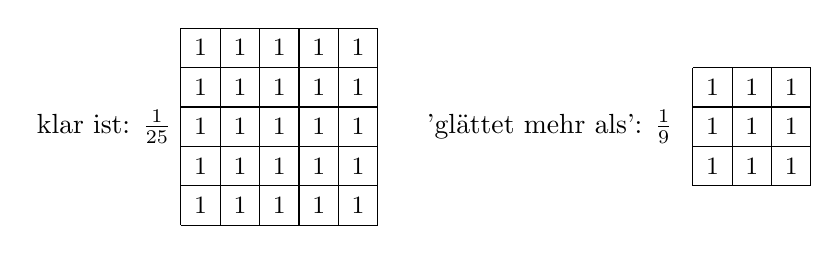
\begin{tikzpicture}
		\foreach \i in {0,...,4}
			\foreach \j in {0,...,4}
				\draw (0.5*\i + 0.25,0.5*\j + 0.25) node[] {\small 1};
		\draw[step = 0.5] (0,0) grid (2.5,2.5);
		\draw (0,1.25) node[left] {klar ist: $\frac{1}{25}$};
		\draw (3,1.25) node[right] {'glättet mehr als': $\frac{1}{9}$};
		\draw[step = 0.5, shift = {(6.5,0.5)}] (0,0) grid (1.5,1.5);
		\foreach \i in {0,...,2}
			\foreach \j in {0,...,2}
				\draw (0.5*\i + 6.75,0.5*\j + 0.75) node[] {\small 1};
	\end{tikzpicture}
\end{center}

Im Kontinuierlichen: Sei $m \in L^1(\R^d)$ und $s > 0$.
Setze 
	$$ m_s(x) := \frac{1}{s^d} m (\frac{x}{s}), \quad x\in \R^d$$

Bsp (in $d =1 $):
\begin{center}
	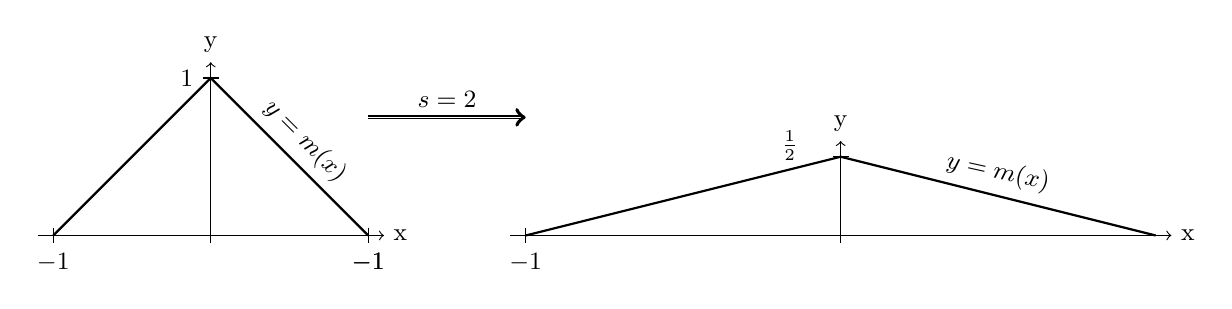
\begin{tikzpicture}
		\draw[->] (-2.2,0) -- (2.2,0) node[right] {\small x};
		\draw[->] (0,-0.1) -- (0,2.2) node[above] {\small y};
		\draw (-2,0.1) -- (-2,-0.1) node[below] {\small $-1$};
		\draw (2,0.1) -- (2,-0.1) node[below] {\small $-1$};
		\draw (0.1,2) -- (-0.1,2) node[left] {\small $1$};
		\draw[thick] (-2,0) -- (0,2) -- (2,0);
		\draw (1.2,1.2) node[rotate = -45] {\small $y=m(x)$};
		\draw[->] (3.8,0) -- (12.2,0) node[right] {\small x};
		\draw[->] (8,-0.1) -- (8,1.2) node[above] {\small y};
		\draw (4,0.1) -- (4,-0.1) node[below] {\small $-1$};
		\draw (2,0.1) -- (2,-0.1) node[below] {\small $-1$};
		\draw (8.1,1) -- (7.9,1) node[left, xshift = -9, yshift = 4] {\small $\frac{1}{2}$};
		\draw[thick] (4,0) -- (8,1) --(12,0);
		\draw (10,0.8) node[rotate = -12.5] {\small $y=m(x)$};
		\draw[->,double] (2,1.5) -- node[above] {\small $s=2$} (4,1.5);
	\end{tikzpicture}
\end{center}

Bsp: Gauß-Kern $G(x) = \frac{1}{(2 \pi)^{\frac{d}{2}}} e^{\frac{-\abs{x}^2}{2}}$\\
Skalierung mit Fehler $s > 0$
$$ \Rightarrow G_s(x) = \frac{1}{s^d} G\left( \frac {x} {s} \right) = \frac{1}{s^d} \frac{1}{(2 \pi)^{\frac{d}{2}}} e^{\frac{-\abs{x}}{2}} = \frac{1}{(2 \pi s^2)^{\frac{d}{2}}} e^{\frac{-\abs{x}^2}{2s^2}}$$

Skalierung $s \hat = $ Standardabweichung $\sigma$
\todoKom{hier noch mehr im Skript p. 45}

\newcommand{\mtitle}[1] {
    \begin{center}
        \large{\textbf{#1}}
    \end{center}
}

\newcommand{\filter}[1] {
	\begin{tabular}{|c|c|c|}
		\hline
		#1\\
		\hline
	\end{tabular}
	}
	

\section{Differenzenfilter}

    Bisher: Glättung $\widehat =$ Mittelwert bilden $\widehat =$ Summe/Integrale\\
    Jetzt: Schärfen $\widehat =$ Differenzen/Kontraste hervorheben $\widehat =$ Differenzen/Ableitungen\\

    \mtitle{Diskretisierung von Ableitungen durch Differenzenquotienten}
    \ \\
    \begin{minipage}[c]{0.25\linewidth}
        \begin{center}
            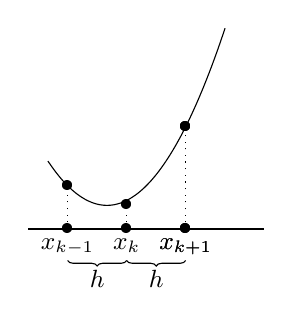
\begin{tikzpicture}
                
                \draw[scale=1,domain=-0.75:1.5,smooth,variable=\x]  plot ({\x},{(\x * \x)});
                \draw[] (-1,-0.3) -- (2,-0.3);
                \draw[dotted] (-0.5,-0.3) node[] {\small \textbullet} node[below] {\small $x_{k-1}$} -- (-0.5,0.25) node[] {\small \textbullet};
                \draw[dotted] (0.25,-0.3) node[] {\small \textbullet} node[below] {\small $x_{k}$} -- (0.25,0.0125) node[] {\small \textbullet};
                \draw[dotted] (1,-0.3) node[] {\small \textbullet} node[below] {\small $x_{k+1}$} -- (1,1) node[] {\small \textbullet};
                \draw[decorate,decoration={brace,amplitude=2pt,mirror}] (-0.5,-0.7) -- node[below] {\small $h$} (0.25,-0.7);
                \draw[dotted] (1,-0.3) node[] {\small \textbullet} node[below] {\small $x_{k+1}$} -- (1,1) node[] {\small \textbullet};
                \draw[decorate,decoration={brace,amplitude=2pt,mirror}] (0.25,-0.7) -- node[below] {\small $h$} (1,-0.7);
            \end{tikzpicture}
        \end{center}
    \end{minipage}
    \hfill\vrule\hfill
    \begin{minipage}[c]{0.4\linewidth}
        (hier bedeutet $f(k) = f(x_k)$)\\
        Vorwärts: $\displaystyle u(h)= \frac{f(k+1) - f(k)}{h}$
        Rückwärts: $\displaystyle u(h)= \frac{f(k) - f(k-1)}{h}$
        Zentral: $\displaystyle u(h)= \frac{f(k+1) - f(k-1)}{2h}$
    \end{minipage}
    \hfill
    \begin{minipage}[c]{0.3\linewidth}
        \ \\
        $u=\displaystyle \frac{1}{h}\begin{tabular}{|c|c|c|}
            \hline
            0 & -1 & 1\\
            \hline
        \end{tabular} \boxast f$\\
        \ \\
        $u=\displaystyle \frac{1}{h}\begin{tabular}{|c|c|c|}
            \hline
            0 & -1 & 1\\
            \hline
        \end{tabular} \boxast f$\\
        \ \\
        $u=\displaystyle \frac{1}{2h}\begin{tabular}{|c|c|c|}
            \hline
            0 & -1 & 1\\
            \hline
            \end{tabular} \boxast f$\\
    \end{minipage}
    \ \\

    \mtitle{2. Abbleitung:}

    \begin{align*}
        u(h) \approx & \frac{f'(k+1) - f'(k)}{h} \text{(vorwärts)}\\
        \approx & \frac{\frac{f(k+1) - f(k)}{h} - \frac{f(k) - f(k-1)}{h}}{h} \text{(rückwärts)} \\
        = & \frac{f(k+1) -2 f(k) + f(k+1)}{h^2}
    \end{align*}

    Also folgt $\displaystyle u:=\begin{tabular}{|c|c|c|}
        \hline
        1 & -2 & 1\\
        \hline
        \end{tabular} \boxast f$ und $\displaystyle \frac{1}{h^2}\begin{tabular}{|c|c|c|}
            \hline
            1 & -2 & 1\\
            \hline
            \end{tabular} = \frac{1}{h}\begin{tabular}{|c|c|c|}
                \hline
                0 & -1 & 1\\
                \hline
                \end{tabular} * \frac{1}{h}\begin{tabular}{|c|c|c|}
                    \hline
                    -1 & 1 & 0\\
                    \hline
                    \end{tabular}$\\
    Denn:

    \begin{align*}
         & \frac{1}{h} \filter{-1 & 1 & 0}\\
        =& \frac{1}{h} \filter{0 & 1 & -1} * \left(\frac{1}{h} \filter{1 & -1 & 0} * f\right)\\
        =& \left(\frac{1}{h} \filter{ 0 & 1 & -1} * \frac{1}{h} \filter{1 & -1 & 0}\right)*f\\
        =& \left(\frac{1}{h} \filter{ -1 & 1 & 0} \boxast \frac{1}{h} \filter{1 & -1 & 0}\right)*f\\
        =& \frac{1}{h^2} \filter{1 & -2 & 1} * f \\
        =&\frac{1}{h^2} \filter{1 & -2 & 1} \boxast f 
    \end{align*}

    In 2D: $\displaystyle \frac{\partial}{\partial x} \widehat = \ \begin{tabular}{|c|c|c|}
        \hline
        0 & -1 & 1\\
        \hline
    \end{tabular}, \ \frac{\partial}{\partial y} \widehat = \begin{tabular}{|c|}
        \hline
        0\\
        \hline
        -1\\
        \hline
        1\\
        \hline
    \end{tabular}, \ \frac{\partial^2}{\partial x^2} \widehat = \begin{tabular}{|c|c|c|}
        \hline
        1 & -2 & 1\\
        \hline
    \end{tabular}, \ \frac{\partial^2}{\partial y^2} \widehat = \begin{tabular}{|c|}
        \hline
        1\\
        \hline
        -2\\
        \hline
        1\\
        \hline
    \end{tabular}$.\\
    \ \\
    \mim{Diskreter Laplace Operator}:
    \[\Delta = \frac{\partial^2}{\partial x^2} + \frac{\partial^2}{\partial y^2} \widehat = \ \begin{tabular}{|c|c|c|}
        \hline
        1 & -2 & 1\\
        \hline
    \end{tabular} + \begin{tabular}{|c|}
        \hline
        1\\
        \hline
        -2\\
        \hline
        1\\
        \hline
    \end{tabular} = \begin{tabular}{|c|c|c|}
        \hline
         0 & 1 & 0\\
        \hline
        1 & -4 & 1\\
        \hline
         0 & 1 & 0\\
        \hline
    \end{tabular}\]

\section{Glättungsfilter und partielle Differentialgleichungen}

    Wir haben gesehen: $\displaystyle m = \frac{1}{5}\begin{tabular}{|c|c|c|}
        \hline
        0 & 1 & 0\\
        \hline
        1 & 1 & 1\\
        \hline
        0 & 1 & 0\\
        \hline
    \end{tabular}$ ist unter allen 5-Punkt Filtern der am besten glättende.\\
    Idee: Rauschen weiter verringern indem man $m \boxast$ wiederholt anwendet $\Rightarrow$ Folge von Bildern:\\
    
    \begin{center}
        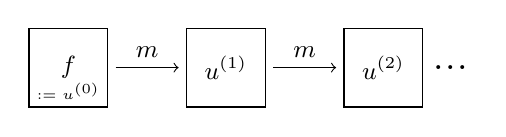
\begin{tikzpicture}
            \draw (0,0) rectangle (1,1);
            \draw (0.5,0.5) node {\small $f$};
            \draw (0.5,0.2) node {\tiny $:= u ^{(0)}$};
            \draw[->] (1.1,0.5) -- node[above] {\small $m \boxast$}(1.9,0.5);
            \draw (2,0) rectangle (3,1);
            \draw (2.5,0.5) node {\small $u^{(1)}$};
            \draw[->] (3.1,0.5) -- node[above] {\small $m \boxast$}(3.9,0.5);
            \draw (4,0) rectangle (5,1);
            \draw (4.5,0.5) node {\small $u^{(2)}$};
            \draw (5,0.5) node[right] {\LARGE ...};
        \end{tikzpicture}
    \end{center}
    
    \begin{align*}
        \Rightarrow u^{(n+1)} - u^{(n)} & = \text{(Unterschied zwischen 'Zeit' Punkt $n$ und $n+1$)}\\
        &= \underbrace{m \boxast u^{(n)}}_{u^{n+1}} - \underbrace{\delta \boxast u^{(n)}}_{u^{(n)}} \text{mit } \delta = \begin{tabular}{|c|c|c|}
            \hline
            0 & 0 & 0\\
            \hline
            0 & 1 & 0\\
            \hline
            0 & 0 & 0\\
            \hline
        \end{tabular}\\
        &=(m - \delta) \boxast u^{(n)}\\
        &=\left( \frac{1}{5}\begin{tabular}{|c|c|c|}
            \hline
            0 & 1 & 0\\
            \hline
            1 & 1 & 1\\
            \hline
            0 & 1 & 0\\
            \hline
        \end{tabular} - \frac{1}{5} \begin{tabular}{|c|c|c|}
            \hline
            0 & 0 & 0\\
            \hline
            0 & 5 & 0\\
            \hline
            0 & 0 & 0\\
            \hline
        \end{tabular}\right) \boxast u^{(n)}\\
        &= \frac{1}{5} \begin{tabular}{|c|c|c|}
            \hline
            0 & 1 & 0\\
            \hline
            1 & -4 & 1\\
            \hline
            0 & 1 & 0\\
            \hline
        \end{tabular} u^{(n)}
    \end{align*}
\begin{equation}
\todomp{noch einmal schauen was 5.10 ist}
\end{equation}
    Somit gilt insgesamt:

    \begin{equation}\label{eq:5.11}
        \underbrace{u^{(n+1)} - u^{(n)}}_{\widehat = \frac{\partial u}{\partial t}} = \underbrace{\frac{1}{5} \begin{tabular}{|c|c|c|}
            \hline
            0 & 1 & 0\\
            \hline
            1 & -4 & 1\\
            \hline
            0 & 1 & 0\\
            \hline
        \end{tabular}}_{\widehat = \Delta u}
    \end{equation}

    Kontinuierlich: Funktion $u$
    \[u(x,t) \quad x \in \R^2, \ t \text{ Zeit} \]

    \eqref{eq:5.11} ist eine Diskretisierung (1 Zeitschritt im Eulerverfahren) der partiellen Differentialgleichungen
    \begin{equation}\label{eq:5.12}
        \frac{\partial u}{\partial t} = \Delta u
    \end{equation}
    Bekannt als \mim{Wärmegleichung} oder \mim{Diffusionsgleichung}.\\
    Zum Zeitpunkt $t=0$ möge die Anfangsbedingung
    \begin{equation}\label{eq:5.13}
        u(x,0)=u^{(0)}=f(x)
    \end{equation}
    gelten. Vorranschreiten der Zeit $t$ repräsentiert Diffusion.\\
    Für einen stationären Zustand, also keine Änderung $\frac{\partial u}{\partial t}$ dann muss auch $\Delta u =0$ gelten.\\
    Diese wird unteranderem von konstanten Funktionen oder linearen Funktionen $u(x_1,x_2) = ax_1 + bx_2$ erfüllt.\\
    \ \\
    Es existiert auch einen explizite Formel für die Lösung der Diffusionsgleichung \eqref{eq:5.12} mit Anfangsbedingung \eqref{eq:5.13}:
    \[u(x,t) = \left( G_{\sqrt{2t}} * u^{(0)} \right)(x)\]
    Wobei $\sqrt{2t}$ für eine Skalierung um diesen Wert steht.\\
    Zu zeigen ist: $\displaystyle \frac{\partial u}{\partial t} = \Delta u$
    \[\frac{\partial}{\partial t}  \left( G_{\sqrt{2t}} * u^{(0)} \right) = \Delta  \left( G_{\sqrt{2t}} * u^{(0)} \right)\]
    \[\overset{\text{mit Satz}}{\Longrightarrow}  \left( \frac{\partial}{\partial t} G_{\sqrt{2t}} \right)* u^{(0)} =  \left( \Delta G_{\sqrt{2t}} \right) * u^{(0)}\]
    Es bleibt somit z.z.: $\frac{\partial}{\partial t} G_{\sqrt{2t}} = \Delta G_{\sqrt{2t}}$.

    \begin{center}
        \begin{tikzpicture}
            \draw (0,1.5) node[left] {$t=0$:};
            \draw (0,0) -- (3,0) node[below] {\small a} -- (3,1) -- (4,1) -- (4,0) node[below] {\small b} -- (7,0);
            \draw (0,-2) node[left] {$t>0$:};
            \draw[shift={(0,-3.5)}] plot [smooth, tension = 0.1] coordinates {(0,0) (2.95,0.05) (3.05,1) (3.95,1) (4.05,0.05) (7,0)};
        \end{tikzpicture}
    \end{center}
    Bemerkenswert ist das, für $t=0$ die Funktion nicht stetig ist, aber für alle $t>0$ die Funktion beliebig oft differenzierbar ist.\\
    \ \\
    Insgesamt lässt sich die Idee darstellen als:

    \begin{center}
        \begin{tikzpicture}
            \draw[->] (0,0) node[left] {\small kontinuierlich:} -- (10,0) node[right] {\small t};

            \draw (1,-0.5) rectangle (2,-1.5);
            \draw (1.5,-1) node {\large $u^{(0)}$};
            \draw (1.5,-1.5) node[below] {\small $u(\cdot,0)$};
            \draw[->] (1.5,-2) -- (1.5,-2.5) -- node[above] {\small $G_{\sqrt{2t}}*$} (8.5,-2.5) -- (8.5,-2);
            \draw (8,-0.5) rectangle (9,-1.5);
            \draw (8.5,-1.5) node[below] {\small $u(\cdot,t)$};

            \draw (0,-4) node[left] {\small diskret:};
            \draw (1,-4) rectangle (2,-5);
            \draw (1.5,-4.5) node[] {\large $u^{(0)}$};
            \draw[->] (2.1,-4.5) -- node[above] {\small $m \boxast$} (2.9,-4.5);
            \draw[shift={(2,0)}] (1,-4) rectangle (2,-5);
            \draw[shift={(2,0)}] (1.5,-4.5) node[] {\large $u^{(1)}$};
            \draw[->,shift={(2,0)}] (2.1,-4.5) -- node[above] {\small $m \boxast$} (2.9,-4.5);
            \draw (6,-4.5) node[] {\LARGE ...};

            \draw[shift={(7,0)}] (1,-4) rectangle (2,-5);
            \draw[shift={(7,0)}] (1.5,-4.5) node[] {\large $u^{(n)}$};
            \draw[->,shift={(5,0)}] (2.1,-4.5) -- node[above] {\small $m \boxast$} (2.9,-4.5);
        \end{tikzpicture}
    \end{center}

\todoKom{Ab hier Livetex 24.11}

Wiederholung Diffusionsgleichung letzte Woche:

\todoKom{Vergleich kontinuierlicher mit dem diskreten Fall.}


\begin{tikzpicture}
  \draw[help lines] (0,0) grid (15,3);
\end{tikzpicture}


\section{Isotrope und anisotrope Diffusion}

Haben gesehen: Glättung/Diffusion verringert rauschen

Aber: Auch Kanten/Details werden verwischt.

Ausweg: Diffusion steuern, so dass sie an Kanten weniger stark glättet. 

\emph{an Kanten} Stellen mit großer Änderungsrate in $x$- oder $y$-Richtung,
oder beides, d.h.:

$$ | \frac {\partial u} {\partial x}|^2 + 
	|\frac {\partial u} {\partial y}|^2 = \norm{
		\begin{pmatrix}
			\frac {\partial u} {\partial x}	\\
			\frac {\partial u} {\partial y}	\\
		\end{pmatrix}	
		}^2[\nabla u]$$


\begin{equation}
\text{Plan:} \nabla u 
	\begin{cases} 
		\text{groß} 	& \df \text{Diffusion } \searrow \\
		\text{klein}	& \df \text{Diffusion normal} \\
	\end{cases}
\end{equation}
Diffusionsgleichung: 
	$$ \frac {\partial u} {\partial t} = \Delta u = 
	\frac {\partial u} {\partial x} \; \frac {\partial u} {\partial x} u
	+ 
	\frac {\partial u} {\partial y} \; \frac {\partial u} {\partial y} u
	=\todomp{\dots} = div (M) (\nabla u)$$ 

Ansatz für $M$:

	\begin{minipage}{0.5\linewidth}
		%
	  \begin{enumerate}[a)]

		  \item	$M = I = 
				\begin{pmatrix}
					1 & 0 \\
					0 & 1 \\
				\end{pmatrix}$ $\df$ übliche Diffusion

			\item $M = g(\norm{\nabla u(x,y)}) \cdot I$
				\begin{itemize}[]
					\item $g(s) = \frac {1} { (\frac {s} {\kappa})^2 +1 }	$ 
						mit Parameter $\kappa > 0$
					\item $\df$ Perona \& Malik (1990)
				\end{itemize}

			\item $M = 
					\begin{pmatrix}
						g(| \frac {\partial u} {\partial x}|)	 & 0 \\	
						0 & g(| \frac {\partial u} {\partial y}|)	\\	
					\end{pmatrix}
				$
			
		\end{enumerate}
		%
	\end{minipage}
	%
	\begin{minipage}{0.6\linewidth}
	 	\begin{tikzpicture}
			\draw[shift={(-0.75,0.75)}] (0,0) node[left] {$\displaystyle g_\kappa(s) = \frac{1}{1+\left(\frac{s}{\kappa}\right)^2}$};
			\draw[scale=1.5,domain=0:3,smooth,variable=\x] plot ({\x},{(1/(1+\x*\x)});
			\draw (0,1.5) node[left] {\small 1};
			\draw[->] (0,-0.5) -- (0,2);
			\draw[->] (0,0) -- (5,0) node[right] {\small $s$};
			\draw[dotted] (1.5,0) node [below] {\small $\kappa$} -- (1.5,0.75);
			\draw[dotted] (0,0.75) node[left] {\small $\frac{1}{2}$} -- (1.5,0.75);
	 	\end{tikzpicture} 
		\begin{itemize}
		  \item Kante mit $\norm{\nabla u} < \kappa$ 
				werden gelättet ($g > \frac{1}{2}$)
			\item Kante mit $\norm{\nabla u} \geq \kappa$
				werden nicht geglättet ($g \leq \frac{1}{2}$)
		\end{itemize}
	\end{minipage}

\todoKom{Bild zu isotrop und anisotrop. (Kann man sich sparen?)}

\newcommand{\vecx}[1][x]{\mathbf{#1}}
Im diskreten Fall:
$\vecx \in \Z^2$ $\vecx_W = \vecx + 
	\begin{pmatrix}
		-1 \\ 0
	\end{pmatrix}
$, usw. 

Sei $M = 
\begin{pmatrix}
	c_1 (\vecx) & 0 \\
	0 & c_1 (\vecx) \\	
\end{pmatrix}$

\newcommand{\x}[0]{
	\boldsymbol{x}
}
\newcommand{\y}[0]{
	\boldsymbol{y}
}

\begin{minipage}{0.5\linewidth}
	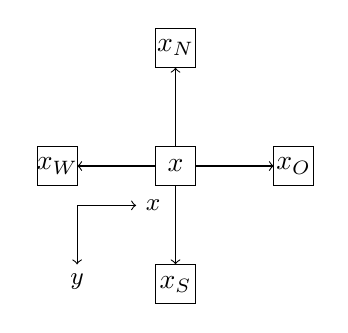
\begin{tikzpicture}
		\draw (0,0) rectangle node[] {$\x$} (0.5,0.5);
		\draw[->] (0.25,0.5) -- ++(0,1);
		\draw (0,1.5) rectangle node[] {$\x_N$} (0.5,2);
		\draw[->] (0.25,0) -- ++(0,-1);
		\draw (0,-1) rectangle node[] {$\x_S$} (0.5,-1.5);
		\draw[->] (0.5,0.25) -- ++(1,0);
		\draw (1.5,0) rectangle node[] {$\x_O$} (2,0.5);
		\draw[->] (0,0.25) -- ++(-1,0);
		\draw (-1,0) rectangle node[] {$\x_W$} (-1.5,0.5);
		\draw[->] (-1,-0.25) -- ++(0.75,0) node[right] {\small $x$};
		\draw[->] (-1,-0.25) -- ++(0,-0.75) node[below] {\small $y$};
	\end{tikzpicture}
\end{minipage}
%
\begin{minipage}{0.5\linewidth}
 $
 	\begin{aligned}
 		div( M \cdot \nabla u(\vecx)) 
			&= ( \frac {\partial } {\partial x} \; 
				\frac {\partial } {\partial x})\left[
				\begin{pmatrix}
					c_1 (\vecx) & 0 \\
					0 & c_2 (\vecx) \\	
				\end{pmatrix}
				\begin{pmatrix}
					\frac {\partial u} {\partial x} (\vecx) \\	
					\frac {\partial u} {\partial y} (\vecx) \\	
				\end{pmatrix}	
			\right] \\
			%
			&= ( \frac {\partial } {\partial x} \; 
				\frac {\partial } {\partial x})
				\begin{pmatrix}
					c_1 (\vecx) \cdot \frac {\partial u} {\partial x} (\vecx)\\
					c_2 (\vecx) \cdot \frac {\partial u} {\partial y} (\vecx)\\	
				\end{pmatrix} \\
			%
			&\approx ( \frac {\partial } {\partial x} \; 
				\frac {\partial } {\partial x})
				\begin{pmatrix}
					c_1 (\vecx) \cdot \todomp{..})\\
					c_2 (\vecx) \cdot \todomp)\\	
				\end{pmatrix} \\
 	\end{aligned}
 $ 
\end{minipage}

\todoKom{Ab hier livetex}
\todoKom{Wiederholung von letzter Woche.}
Bei Salt, Pepper einmal vorglätten, aber nur bei der $u$ in der Steuerungsfunktion.


\section{Bilaterale Filter}

Anderer Ansatz für selbes Problem:
	$$ u (\vecx) := \text{gewichtetes Mittel aus allen } f(\vecx[y]) \text{ mit}$$

	\begin{enumerate}[a)]
	  \item $\vecx[y]$ ist nahe bei $\vecx$ \emph{und}
		\item $f(\vecx[y])$ ist nahe bei $f(\vecx)$
	\end{enumerate}

	$$ u(\vecx)  = \frac {1} {w(\vecx)} \int_\Omega g(\norm{|\vecx - \vecx[y]|}) 
		f(\vecx[y]) d\vecx[y] \todomp{unterpunkte}$$

	Oft: $g,h$ \dots Gauß-Kerne ($\df$ \enquote{nichtlinearer Gauß-Filter})

	Manchmal: $g,h$ \dots charakteristische Funktionen \todomp{bild}.
	($\df$ \enquote{SUSAN-Filter}) 
	\todomp {oder Mischunngen}

	Effekt: Falls Höhe (Kante) > Filterradius ($h$) $\df$ Kante bleibt erhalten.

	Numerische sehr aufwändig:
		\begin{itemize}[-]
		  \item keine reine Faltung ($\df$ keine FFT-Implementierung möglich) 
			\item Normierung $w(\vecx)$ in jedem Punkt neu berechnen.
		\end{itemize}

Manchmal: $f \overset{\log}{\mapsto} \log f \overset{\text{bil Filter}}{\mapsto}
	\log u \overset{\exp}{\mapsto} u$
	
\section{Entrauschen mittels Variationsrechnung}

Erinnerung: $\todomp{Bild}$

\begin{enumerate}[{Wunsch} 1:]
  \item $u \approx f$ \hfill (Datenkonsistenz)
	\item $u$ sei \enquote{glatt} (Regularitätsbedingung)
\end{enumerate}

Mathematische Umsetzung der Wünsche:

\begin{enumerate}[{Wunsch} 1:]
  \item $\norm{u -f}_2 = \sqrt{\int_\Omega |u(x) - f(x)|^2 dx}$ sei klein. 
	\item $ \norm{\nabla u}_2 = \sqrt{\int_\Omega |\nabla u(x)|^2 dx} 
		= \sqrt{\int_\Omega ( \frac {\partial u} {\partial x} (x)^2) + 
		( \frac {\partial u} {\partial y} (x)^2) dx}$ sei klein
\end{enumerate}

Kombination:  

\begin{equation}
\label{5.15}
\norm{u -f}_2 + \lambda \cdot \norm{\nabla}_2^2 
	\overset{u\in U}{\longrightarrow} \min
\end{equation}

	U \dots geeigneter Funktionenraum

	$\lambda > 0$, fest (\enquote{Kopplungskonstante})	

In diesem Bsp. empfiehlt sich als Suchraum

$$ U = \set{ u: \norm{u}_2 < \infty, \nabla u \text{ existiert }, 
\norm{\nabla u}_2 < \infty} =: W^{1,2}[]
$$

1 \dots Ableitung 1. Ordnung

2 \dots 2-Norm

Im obigen Ansatz (\ref{5.15}) stellt man fest, dass der Regularitätsterm

	$$ \norm{\nabla u}_2^2 = {\int_\Omega |\nabla u(x)|^2 dx} 
		= {\int_\Omega ( \frac {\partial u} {\partial x} (x)^2) + 
		( \frac {\partial u} {\partial y} (x)^2) dx}$$

die große Gradiente an (gewollten Kanten) zu stark bestraft. 
($\df$ optimales $u$ hat geglättete Kanten)

Ausweg: Wähle $\norm{\nabla u}_2 = \sqrt {s.o.}$ oder 
$\norm{\nabla u}_1 = \int |\nabla u(x)| dx 
= \int_\Omega ( |\frac {\partial u} {\partial x} (x)| 
+ |\frac {\partial u} {\partial y} (x)| ) dx$

\begin{equation}
\label{5.16}
\norm{u -f}_2 + \lambda \cdot \norm{\nabla}_1 
	\overset{u\in U}{\longrightarrow} \min
\end{equation}
